\documentclass[11pt]{article}
\usepackage{euscript}

\usepackage{amsmath}
\usepackage{amsthm}
\usepackage{amssymb}
\usepackage{epsfig}
\usepackage{xspace}
\usepackage{color}
\usepackage{url}

%%%%%%%%%%%%%%%%%%%%%%%%%%%%%%%%%
\setlength{\textheight}{9in}
\setlength{\topmargin}{-0.600in}
\setlength{\headheight}{0.2in}
\setlength{\headsep}{0.250in}
\setlength{\footskip}{0.5in}
\flushbottom
\setlength{\textwidth}{6.5in}
\setlength{\oddsidemargin}{0in}
\setlength{\evensidemargin}{0in}
\setlength{\columnsep}{2pc}
\setlength{\parindent}{1em}
%%%%%%%%%%%%%%%%%%%%%%%%%%%%%%%%%


\newcommand{\eps}{\varepsilon}

\renewcommand{\c}[1]{\ensuremath{\EuScript{#1}}}
\renewcommand{\b}[1]{\ensuremath{\mathbb{#1}}}
\newcommand{\s}[1]{\textsf{#1}}

\newcommand{\E}{\textbf{\textsf{E}}}
\renewcommand{\Pr}{\textbf{\textsf{Pr}}}

\title{Homework Form for Data Mining
\footnote{\s{CS 6955 Data Mining; \;\; Spring 2012 \hfill
Instructor: Jeff M. Phillips, University of Utah}
}
}
\author{Alex Clemmer}

\begin{document}
\maketitle





%%%%%%%%%%%%%%%%%%%%%%%%%%%%%%%%%%%%%%%%%%%%%%%%%%%%
%%%%%%%%%%%%%%%%%%%%%%%%%%%%%%%%%%%%%%%%%%%%%%%%%%%%
%%%%%%%%%%%%%%%%%%%%%%%%%%%%%%%%%%%%%%%%%%%%%%%%%%%%
\section{Overview}

This is a sample latex file to use for completing assignments.  This particular file is not required.  In fact, there are many cool ways to spruce up this plain look.  Feel free to use them.  

\section{Q1: Birthday ``Paradox"}

\paragraph*{A:} For domain $n = 1000$, it took 58 random trials.

\paragraph*{B:} Please see figure \ref{fig:cdp1}.

\begin{figure}[h]
\centering{
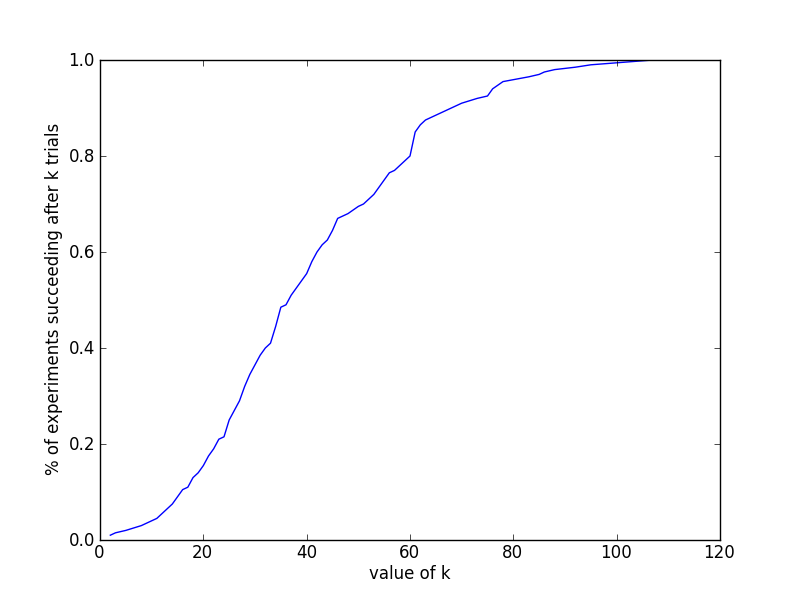
\includegraphics[width=.6\linewidth]{fig1.png}
}
\caption{The \% of experiments requiring $k$ tests before collision, plotted as a function of $k$.}
\label{fig:cdp1}
\end{figure}

\paragraph*{C:} For some $m = 200$ random variables $X_1 \ldots X_m$ representing the outcomes of $m$ random repetitions of the experiment, the expected value $\E[\vec{X}] = 38.005$

\paragraph*{D:} 

I check uniqueness using a bit vector of length $n$, where each place is 0 if we haven't seen the corresponding element before, and is 1 if we have. As long as this bit vector fits in memory, it should scale pretty well. This is probably roughly optimal for exact solutions, though for approximate solutions, you might be able to relax the memory constraint.

The algorithm as coded should run in at most linear time on $n$, but in practice, it runs sublinearly. In figure \ref{fig:runningtimes}, we show that even when we exponentially increase $m$  Extending the domain $n$ should not majorly impact run time as long as we assume $n$ is small enough to fit in the traditional constant-time operations. If you're curious, I've plotted the running time as we increase $m$ exponentially, noted by figure \ref{fig:runningtimes}. It looks to be sub-linear, at least as long as we're assuming constant-time operations.


\begin{figure}[h]
\centering{
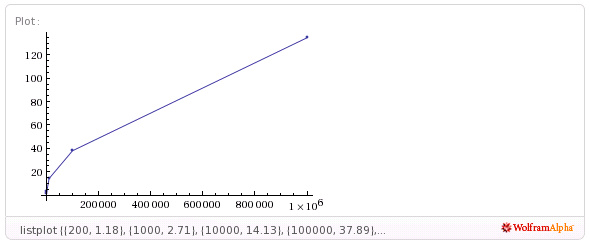
\includegraphics[width=.6\linewidth]{fig2.png}
}
\caption{The running time ($x$-axis) increases by successive powers of 10; the $y$-axis denotes the running time of seconds it took to complete.}
\label{fig:runningtimes}
\end{figure}


\section{Q2: Coupon Collectors}

\paragraph*{A:} For the domain $n = 60$, the required trials $k = 198$.

\paragraph*{B:} As we can see in figure \ref{fig:hist}, the highest bar was pinged 10 times.

\begin{figure}[h]
\centering{
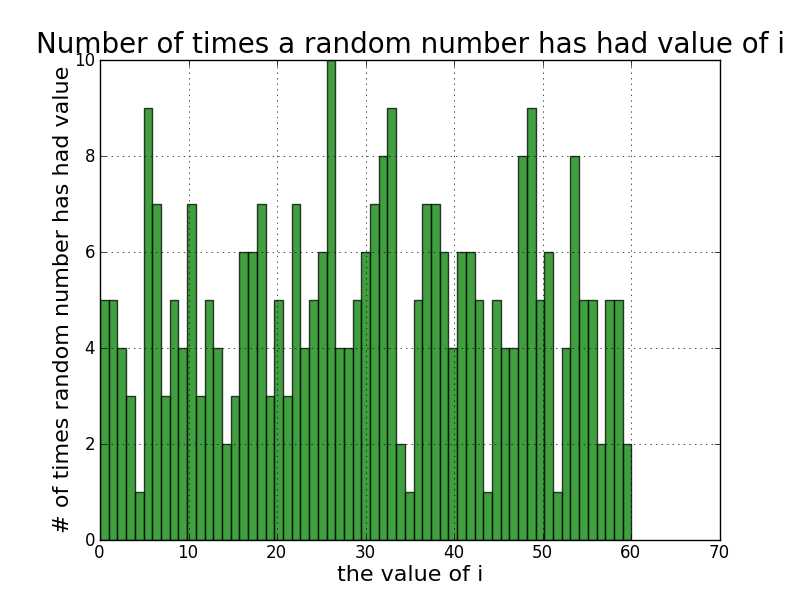
\includegraphics[width=.6\linewidth]{fig3.png}
}
\caption{The number of times a random number ends up with value $i$.}
\label{fig:hist}
\end{figure}

\paragraph*{C:} Please see figure \ref{fig:cdp2}.

\begin{figure}[h]
\centering{
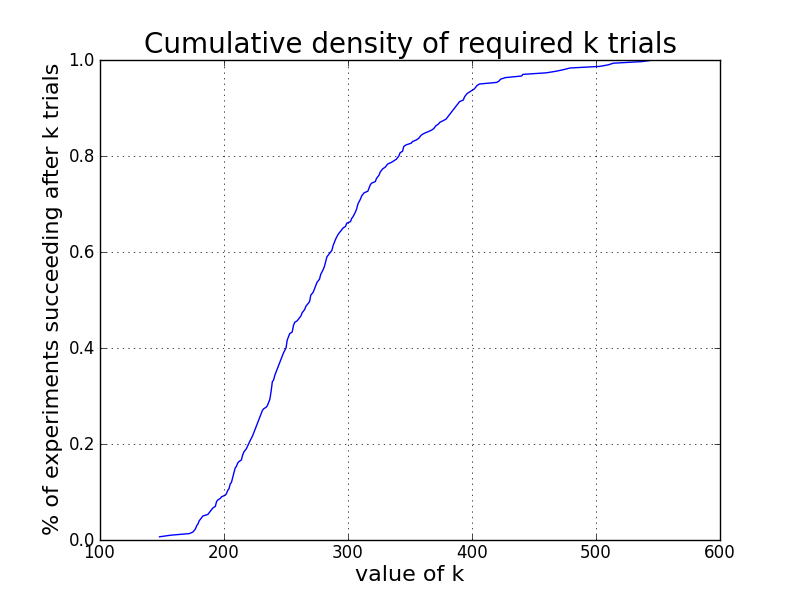
\includegraphics[width=.6\linewidth]{fig4.png}
}
\caption{The number of times a random number ends up with value $i$.}
\label{fig:cdp2}
\end{figure}

\paragraph*{D:} For some $m = 300$ random variables $X_1 \ldots X_m$ representing the outcomes of $m$ random repetitions of the experiment, the expected value $\E[\vec{X}] = 283.61$

\paragraph*{E:} I implemented this on a streaming basis.




\end{document}
